%%%%%%%%%%%%%%%%%%%%%%%%%%%%%%%%%%%%%%%%%%%%%%%%%%%%%%%%%%%%%%%%%%%%%%%%%%%%%%%%
%2345678901234567890123456789012345678901234567890123456789012345678901234567890
%        1         2         3         4         5         6         7         8

\documentclass[letterpaper, 10 pt, conference]{ieeeconf}  % Comment this line out
                                                          % if you need a4paper
%\documentclass[a4paper, 10pt, conference]{ieeeconf}      % Use this line for a4
                                                          % paper

\IEEEoverridecommandlockouts                              % This command is only
                                                          % needed if you want to
                                                          % use the \thanks command
\overrideIEEEmargins
% See the \addtolength command later in the file to balance the column lengths
% on the last page of the document

\usepackage[english]{babel}
\usepackage{graphicx}
\usepackage[style=ieee,backend=bibtex]{biblatex}

% The following packages can be found on http:\\www.ctan.org
%\usepackage{graphics} % for pdf, bitmapped graphics files
%\usepackage{epsfig} % for postscript graphics files
%\usepackage{mathptmx} % assumes new font selection scheme installed
%\usepackage{times} % assumes new font selection scheme installed
%\usepackage{amsmath} % assumes amsmath package installed
%\usepackage{amssymb}  % assumes amsmath package installed

\title{\LARGE \bf
Utilizing Data Mining Techniques to Rethink Saffir-Simpson for Tropical System Landfalls
}

%\author{ \parbox{3 in}{\centering Huibert Kwakernaak*
%         \thanks{*Use the $\backslash$thanks command to put information here}\\
%         Faculty of Electrical Engineering, Mathematics and Computer Science\\
%         University of Twente\\
%         7500 AE Enschede, The Netherlands\\
%         {\tt\small h.kwakernaak@autsubmit.com}}
%         \hspace*{ 0.5 in}
%         \parbox{3 in}{ \centering Pradeep Misra**
%         \thanks{**The footnote marks may be inserted manually}\\
%        Department of Electrical Engineering \\
%         Wright State University\\
%         Dayton, OH 45435, USA\\
%         {\tt\small pmisra@cs.wright.edu}}
%}

\author{Neelesh Rastogi$^{1}$ and Sean Lukasiewicz$^{1}$% <-this % stops a space
\thanks{*This work was supported by St. John's University Data Innovation Lab.}% <-this % stops a space
\thanks{$^{1}$Under guidance of Dr. Christoforos Christoforou, who is with Faculty of Data Mining and Predictive Analytics, Computer Science, Mathematics and Science,
        St. John's University, 8000 Utopia Pkwy, Queens, NY - 11439
        {\tt\small christoc@stjohns.edu}}%
}

\begin{document}

\maketitle
\thispagestyle{empty}
\pagestyle{empty}


%%%%%%%%%%%%%%%%%%%%%%%%%%%%%%%%%%%%%%%%%%%%%%%%%%%%%%%%%%%%%%%%%%%%%%%%%%%%%%%%
\begin{abstract}
The Saffir-Simpson scale is the most well known system through which hurricanes are rated based on the intensity of sustained winds within the storm. It is a simple system placing the storms into six numbered categories and is often the first statement made when talking about the potential impact of a tropical storm. However, as more landfall events occur, we are seeing that the intensity of the wind is not always indicative of the potential impact a storm may have. Hurricane Michael in 2018 and Hurricane Sandy in 2012 both caused approximately \$70 billion in damages to the continental US, but Michael was a Category 4 storm and Sandy was a Category 1 at their respective landfalls.

\end{abstract}
%%%%%%%%%%%%%%%%%%%%%%%%%%%%%%%%%%%%%%%%%%%%%%%%%%%%%%%%%%%%%%%%%%%%%%%%%%%%%%%%

\section{METHODOLOGY}

\subsection{DATA COLLECTION}
The bulk of the data used for this analysis came from open source R packages published by the National Oceanic and Atmospheric Administration (NOAA) and by Dr. Brooke Anderson of Colorado State University’s (CSU) Department of Environmental and Radiological Health Sciences. Other attributes, such as moon phase and tidal data, came from various NOAA webpages and factors used in deriving and normalizing cost coming from the U.S Bureau of Labor Statistics website. Since most of the data is available through R packages, it was natural to use the language for the data collection and pre-processing.

\\The data was collected in a data frame utilizing the \enquote{storm\_id} attribute from CSU's \textit{hurricaneexposuredata} package as the index key. This attribute uses \enquote{name-year} format, and since all storms involved in this analysis occurred after the practice of naming storms started, this provides a unique key that is simple to use. We utilized the \textit{separate} function in R to split the \enquote{DateTime} attribute in the \textit{HURDAT} package into \enquote{Year}, \enquote{Month} and \enquote{Day}; and then the \textit{paste} function to concatenate the \enquote{Name} and \enquote{Year} attributes into the \enquote{storm\_id.} The \textit{merge} function then allowed us to create our table for analysis. Tidal data and moon phase were entered manually from the NOAA Tides and Currents product webpage and the Almanac.com moon phase calendar respectively. Any data further missing from our data frame were manually entered from the official storm report PDFs available on the NOAA website. Microsoft Excel was used to manually input the data.


\subsection{PRE-PROCESSING}
To account for the natural variations within a storm’s track, we opted to derive an effective land speed and effective angle of impact to land. This accounts for any sudden acceleration or change in direction that may occur once a system starts to interact with land. Since the NOAA monitors a system in six-hour intervals, we looked at the twelve-hour window around the moment of landfall to create the displacement vector for this time frame. This displacement vector can be considered to be average velocity of the system from which we can take the effective land speed and effective direction of travel.

\begin{equation}
{\scriptstyle
\mathrm{v}=\frac{\sqrt{\left(62.17^{*} \Delta \mathrm{Latitude}\right)^{2}+\left(69.17^{*} \mathrm{cos}\left(\text { Latitude }_{2}\right) * \Delta \mathrm{Longitude}\right)^{2}}}{12}
}
\end{equation}

\begin{equation}
{\scriptstyle
\text {Angle}=\arctan \left(\frac{\left(69.17 * \cos \left(\text {Latitude}_{2}\right) * \Delta Longitude\right)}{(69.17 * \Delta Latitude)}\right)
}
\end{equation}

The lunar cycle is approximately 28 days long; therefore, the moon phase can be simplified to a discrete scale of 0 to 27, where 0 is a full moon, 14 is a new moon, and 7 and 21 are half-moons. The effects on tidal ranges by moon phase are maximized during the full and new moon phases and minimized on the half-moon. This means that for every lunar cycle the tidal effect goes through two compete cycles. To handle this, we translated the data by subtracting 14 and taking the absolute value. We repeated this process again, this time subtracting by 7, to create a linear scale where 0 is the minimal tidal range and 7 is the maximum range.

\begin{figure}[h!]
  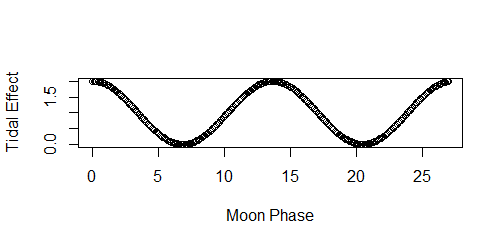
\includegraphics[width=\linewidth]{tidal_plot.png}
  \caption{Effect of moon phase on tidal range}
  \label{fig:tidal}
\end{figure}

The cost of the landfall events were normalized by using yearly consumer price index (CPI) values and state standard of living indices. The cost of each storm \textit{j} was multiplied by the ratio of the 2018 CPI to the CPI of the year the storm occurred to account for inflation then divided by the average cost of living index value of the states affected to account for location.

\begin{equation}
{\scriptstyle
 Cost_{Norm}  =   \frac{\frac{CPI_{2018}}{CPI}* Cost_{j}}{( \Sigma ({Cost of Living}) )/{n} } }
\end{equation}
 Our scale structure came from a visual analysis of the plot of the normalized cost of each landfall event ordered from low to high. This revealed a curve that appeared exponential in nature, so we opted for a base-ten logarithmic scale similar to the Richter magnitude scale, where each point is ten times greater than the previous one. This also produced the most even distribution of events along the scale.  

\subsection{EXPLORATORY DATA ANALYSIS}
Once the data was gathered, and pre-processed, a raw consolidated data file was generated and was further fed into a data frame (df) using pandas. With later df, implicit data values such as effective land speed, effective angle of impact, normalized cost and moon phase were derived and calculated. These calculations were carried out based on equations as mentioned in prior section. Our final Data frame consisted of the following values as shown in Table \ref{table:allfeat}. These values were then, utilized to find common patterns and observations.

\begin{table}[ht]
\caption{All features of our final data frame.}
\centering
\begin{tabular}{|l|l|}
\hline
\textbf{Feature Name} & \textbf{Feature Type} \\ \hline
storm\_names & 115 non-null object \\ \hline
eff\_land\_sp & 115 non-null float64 \\ \hline
direct & 115 non-null int64 \\ \hline
angled & 115 non-null int64 \\ \hline
cross & 115 non-null int64 \\ \hline
press\_mbars & 115 non-null int64 \\ \hline
max\_sust\_winds\_kts & 115 non-null int64 \\ \hline
storm\_surge & 115 non-null float64 \\ \hline
storm\_tide & 115 non-null float64 \\ \hline
moon\_phase & 115 non-null int64 \\ \hline
low\_neap & 115 non-null int64 \\ \hline
high\_neap & 115 non-null int64 \\ \hline
high\_ebb & 115 non-null int64 \\ \hline
high\_tide\_line & 115 non-null float64 \\ \hline
low\_tide\_line & 115 non-null float64 \\ \hline
norm\_cost & 115 non-null float64 \\ \hline
cost\_category & 115 non-null category \\ \hline
\end{tabular}
\label{table:allfeat}
\end{table}

Our data set is comprised of all landfall events along the North American Atlantic and Gulf Coast basins between the years of 1985 and 2017. The location of these events can be seen in Figure \ref{fig:storm_us}

\begin{figure}[h!]
  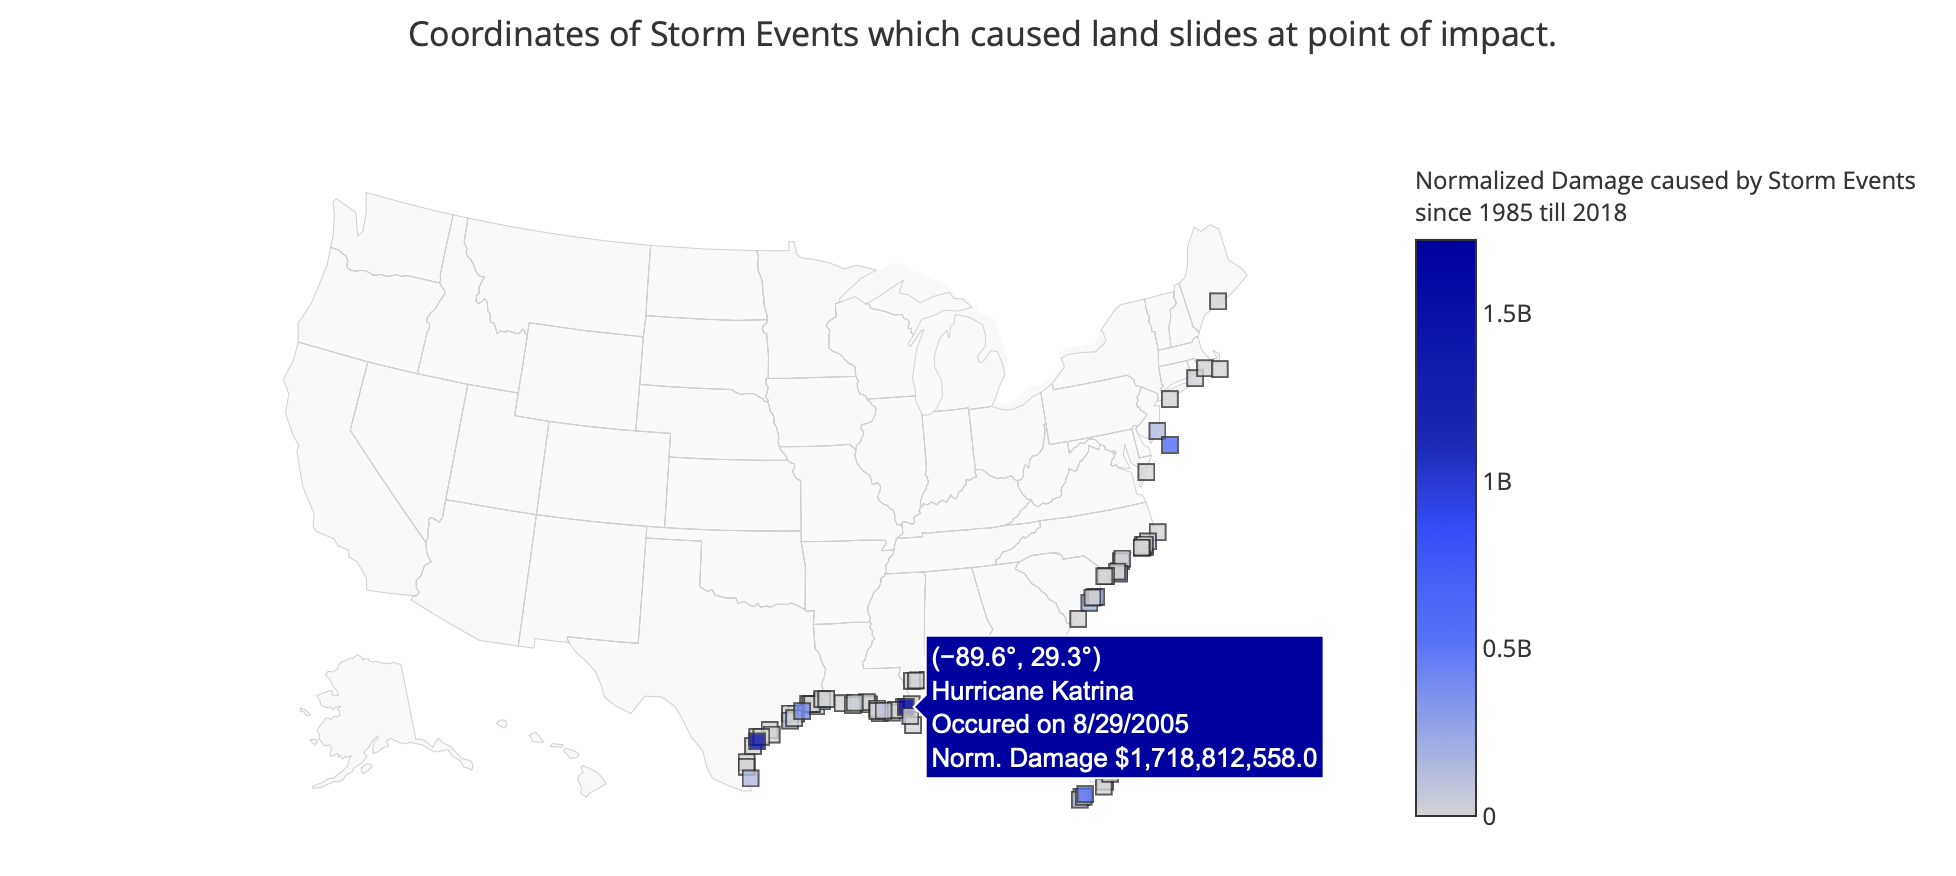
\includegraphics[width=\linewidth]{us_map.png}
  \caption{All Storm events plotted via coordinates since 1985 - 2017.}
  \label{fig:storm_us}
\end{figure}

On an initial analysis we found the following observations:
\begin{itemize}
\item Our current curated data-set currently consists of in total 115 storms, out of which we observed our data set having 48 storms which caused minimal damage and around 34 storms which caused severe to catastrophic level damage. Table \ref{table:stormcountsdamage} below shows all storm counts for all levels of damage caused during landfall. 
\end{itemize}

\begin{table}[ht!]
\caption{Count of all storms based on their damage.}
\centering
\begin{tabular}{|l|l|}
\hline
minimal      & 48 \\ \hline
low          & 6  \\ \hline
moderate     & 8  \\ \hline
high         & 19 \\ \hline
severe       & 17 \\ \hline
catastrophic & 17 \\ \hline
\end{tabular}
\label{table:stormcountsdamage}
\end{table}

\begin{itemize}
\item  On grouping our data-set by year of storm events, we observed Most storms occurred in the year of 2004 followed by year 1998 and 2005. The frequency chart is shown below in Figure \ref{fig:storm_year}

\end{itemize}

\begin{figure}[h!]
  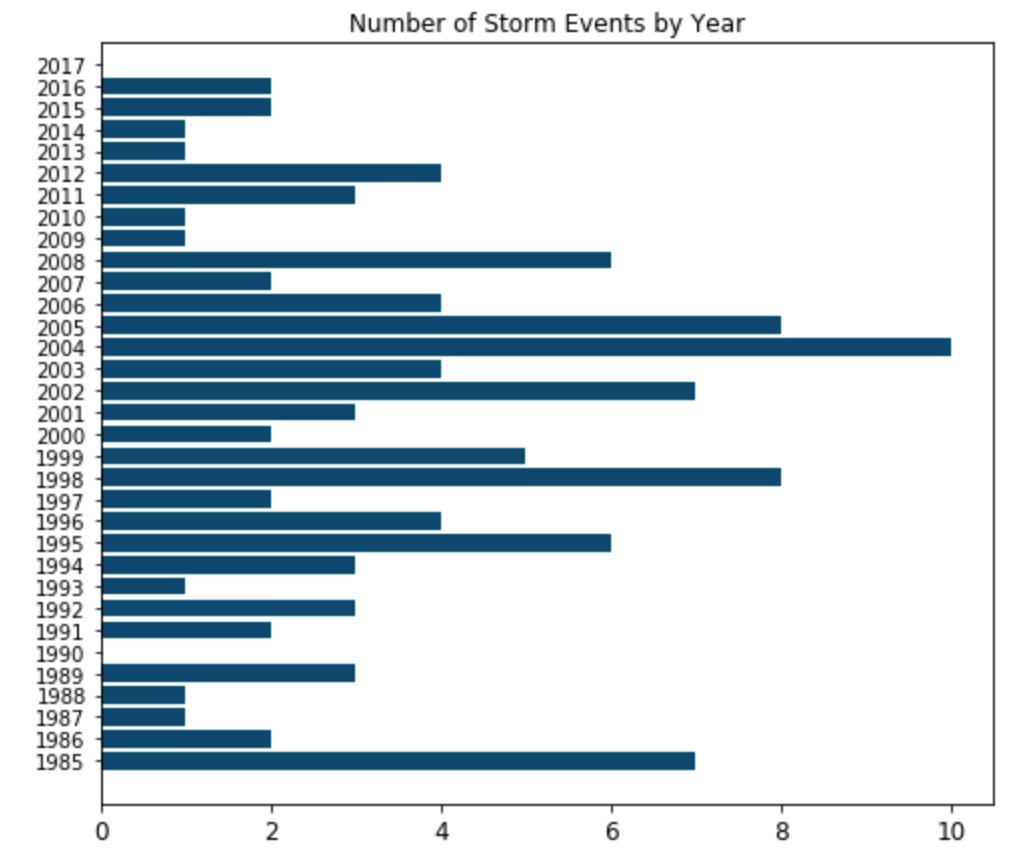
\includegraphics[width=\linewidth]{year_freq.png}
  \caption{Number of Storm Events by Year.}
  \label{fig:storm_year}
\end{figure}

%
%\begin{itemize}
%    \item We also observed that all storms occurred between the season months of May to %October, making the month of August and September more prone to Landfall causing storms %events. This can further be seen visually in Figure  \ref{fig:storm_month}
%\end{itemize}

%\begin{figure}[h!]
%  \includegraphics[width=\linewidth]{month_freq.png}
%  \caption{Number of Storm Events by Month.}
%  \label{fig:storm_month}
%\end{figure}
%

\subsection{CLASSIFICATION}

\begin{table*}[t]
\caption{Comparison of all accuracies and mse's means and std. dev. achieved.}
\centering
\begin{tabular}{|l|l|l|l|l|l|l|l|l|}
\hline
\multicolumn{5}{|l|}{\textbf{MSE Comparison}}                                                                                 & \multicolumn{4}{l|}{\textbf{Accuracy Comparison}}                                              \\ \hline
\textbf{}                    & \multicolumn{2}{l|}{\textbf{Our Dataset}} & \multicolumn{2}{l|}{\textbf{Saffir Simpson Model}} & \multicolumn{2}{l|}{\textbf{Our Dataset}} & \multicolumn{2}{l|}{\textbf{Saffir Simpson Model}} \\ \hline
\textbf{Models}              & Mean                 & Std dev            & Mean                     & Std dev                 & Mean                & Std dev             & Mean                     & Std dev                 \\ \hline
\textit{Decision Trees}      & 4.21E+00             & 5.4E-01            & 4.605263                 & 1.81E-15                & 0.514431            & 3.52E-02            & 0.447368                 & 1.69E-16                \\ \hline
\textit{KNN}                 & 6.55E+00             & 9.0E-16            & 6.684211                 & 9.03E-16                & 0.394737            & 1.13E-16            & 0.342105                 & 1.69E-16                \\ \hline
\textit{Logistic Regression} & 4.68E+00             & 9.0E-16            & 4.394737                 & 1.81E-15                & 0.421053            & 2.82E-16            & 0.421053                 & 2.82E-16                \\ \hline
\textit{Random Forest}       & 4.26E+00             & 6.8E-01            & 5.312281                 & 1.12E+00                & 0.489813            & 6.18E-02            & 0.428947                 & 3.73E-02                \\ \hline
\textit{SVM}                 & 4.84E+00             & 1.8E-15            & 6.631579                 & 1.81E-15                & 0.447368            & 1.69E-16            & 0.421053                 & 2.82E-16                \\ \hline
\textit{XGBoost}             & 4.55E+00             & 9.0E-16            & 4.973684                 & 1.81E-15                & 0.578947            & 1.13E-16            & 0.447368                 & 1.69E-16                \\ \hline
\end{tabular}
\label{table:accvsmse}
\end{table*}

Once we identified our initial observations within exploratory data analysis, we then conducted supervised machine learning processes to identify significant traits within storm systems to identify top features for predicting potential storm damage and potential cost incurred after landfall.

We initially ran an ensemble of classification models like XGBoost, Support Vector Machines, Random Forest, Decision Tree, K-Nearest Neighbor and Logistic Regression on our curated data set, which was randomly split in 70-30 ratio with a parameter of \texttt{(random\_state = 40)}, and was further looped for a total of 30 iterations, giving us 30 unique accuracies and mean squared errors for all our 6 models. The similar procedure was replicated over Saffir-Simpson scale which solely relied of maximum sustained wind speed as its training variable. Below table \ref{table:accvsmse} shows the mean and standard  deviation of all accuracies and mean squared errors achieved through this process.

The above mentioned classification algorithms took 80 historic storm events as its input and was further tested on the other 35 tropical system landfalls. The results of all models were then compared to Saffir-Simpson’s output with all of  our data models showing improvement over Saffir-Simpson. Our best individual  model was found to be Decision Tree Classifier with an mean accuracy of 51.44 percent\% compared to Saffir Simpson Scale, which was  44.74\% accuracy.

\subsection{FEATURE OPTIMIZATION}
Based on our findings we then ran a Recursive Feature Elimination process along with a 5 fold cross validation, over our selected model of Decision Tree Classifier. 

Recursive Feature Elimination (RFE) is a feature selection method that fits a model and removes the weakest feature (or features) until the specified number of features is reached. Features are ranked by the model’s coef\_ or feature\_importances\_ attributes, and by recursively eliminating a small number of features per loop, RFE attempts to eliminate dependencies and cl-linearity that may exist in the model.

\begin{figure}[h!]
  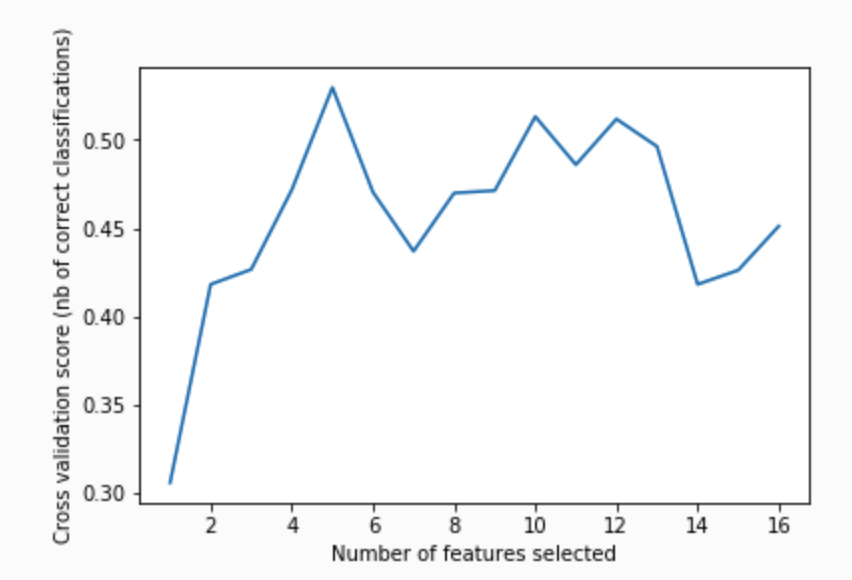
\includegraphics[width=\linewidth]{optimal_feat.png}
  \caption{Optimal Number of Features.}
  \label{fig:optimal_feat}
\end{figure}

As, RFE requires a specified number of features to keep, cross-validation is used with RFE to score different feature subsets and select the best scoring collection of features.

Based on the findings, as shown in Figure \ref{fig:optimal_feat}f 5 features were found to be the optimal number.

\begin{figure}[h!]
  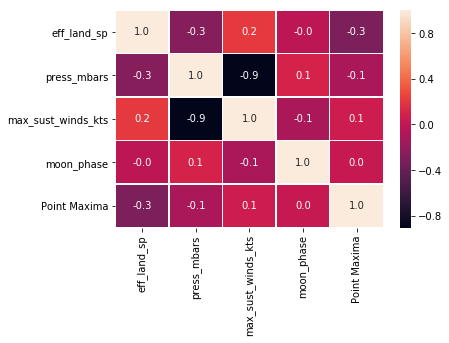
\includegraphics[width=\linewidth]{corr.png}
  \caption{Correlation Values between each Feature pairs.}
  \label{fig:corr}
\end{figure}

These 5 optimal features were:, Point\_Maxima, moon\_phase, max\_sust\_winds\_kts, press\_mbars and eff\_land\_sp. A pair grid analysis as shown in Figure \ref{fig:pairgrid} and \ref{fig:corr}, shows  us a linear relationship between moon phase and other features. Also most of these feature points seemed to be clustered closely as well, when plotted in pairs.

\begin{figure}[h!]
  \centering
  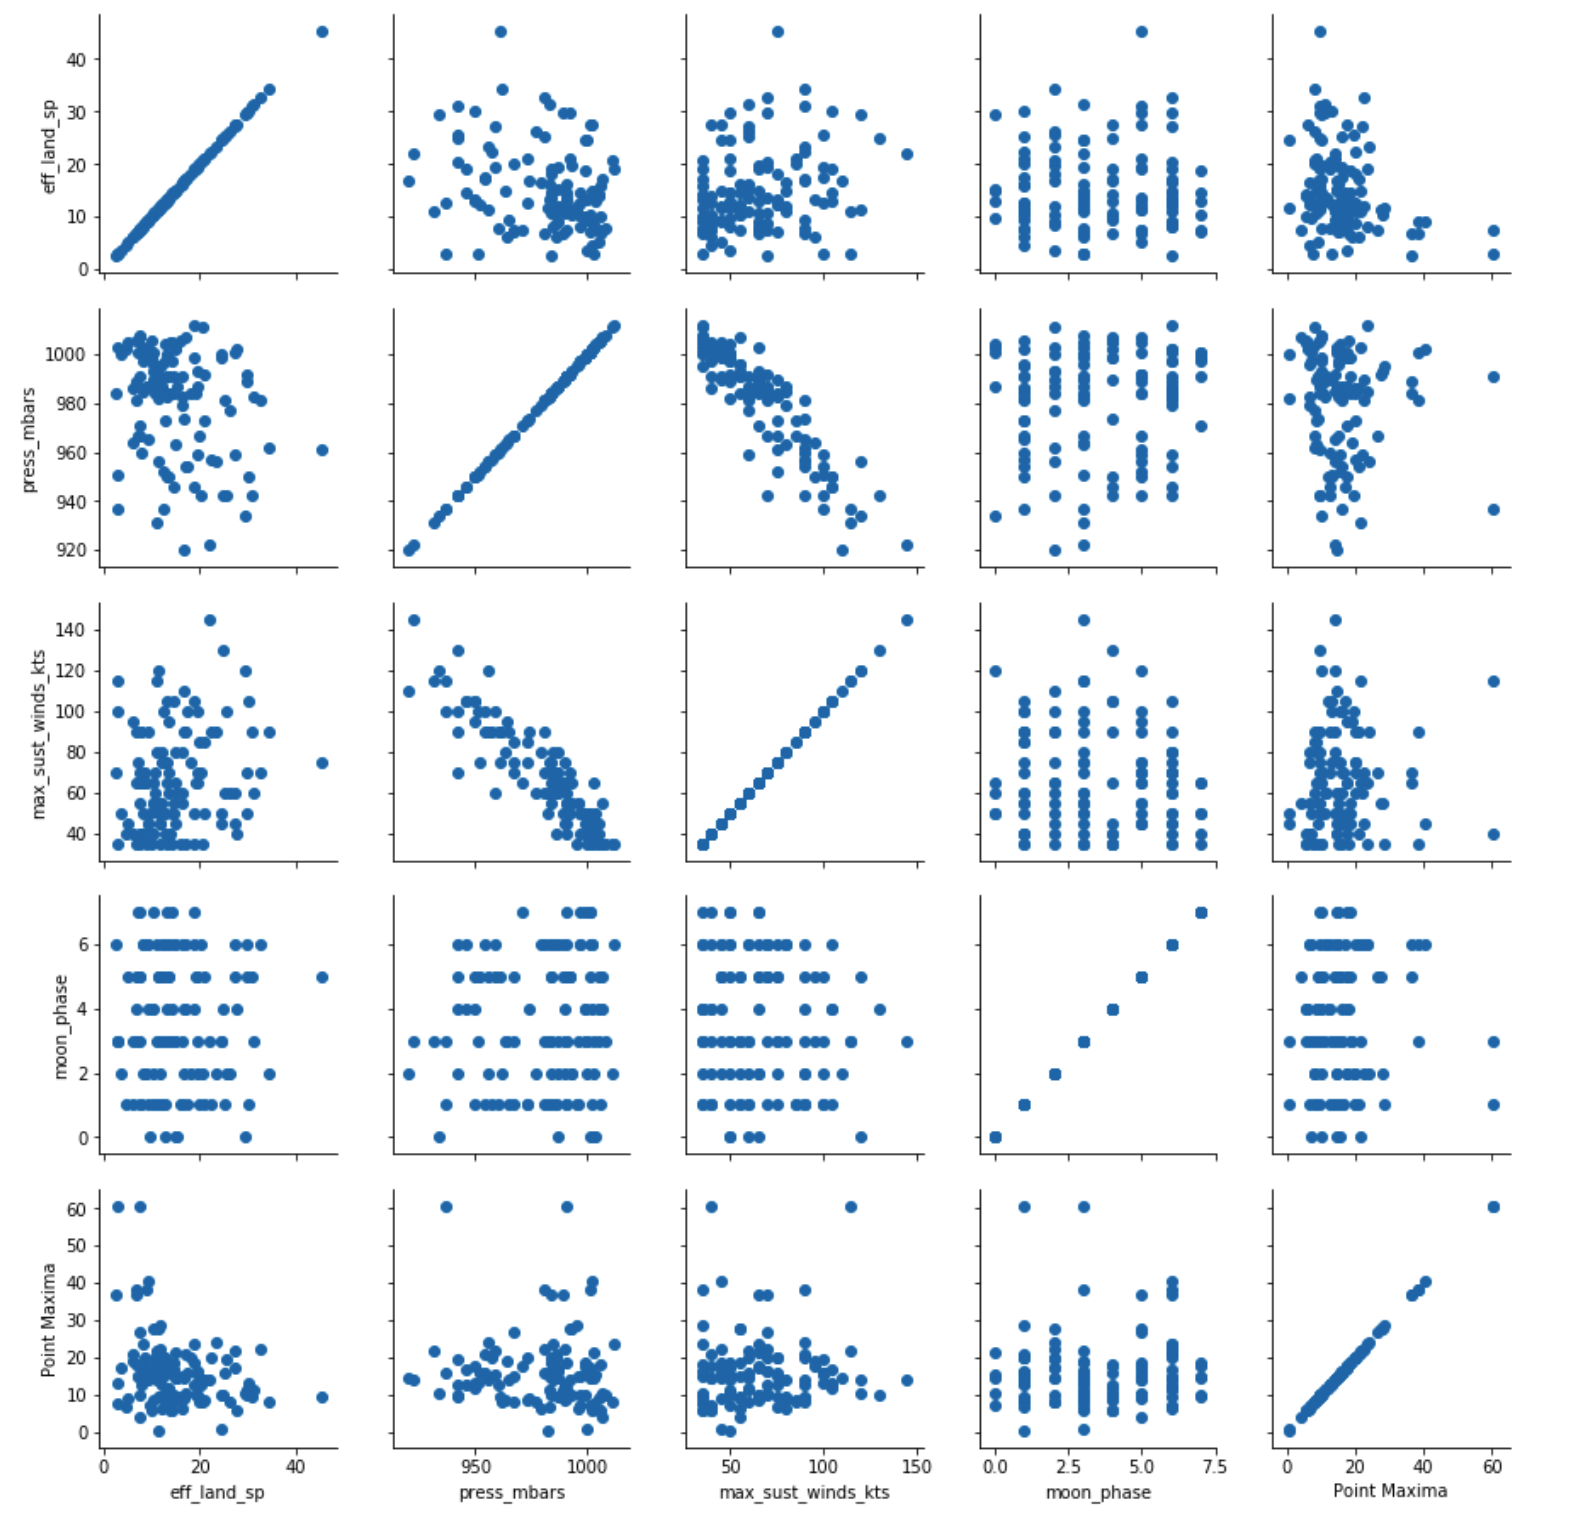
\includegraphics[width=0.7\columnwidth]{pair_grid.png}
  \caption{Pair Grid between each Feature pairs.}
  \label{fig:pairgrid}
\end{figure}

\begin{figure*}[h!]
  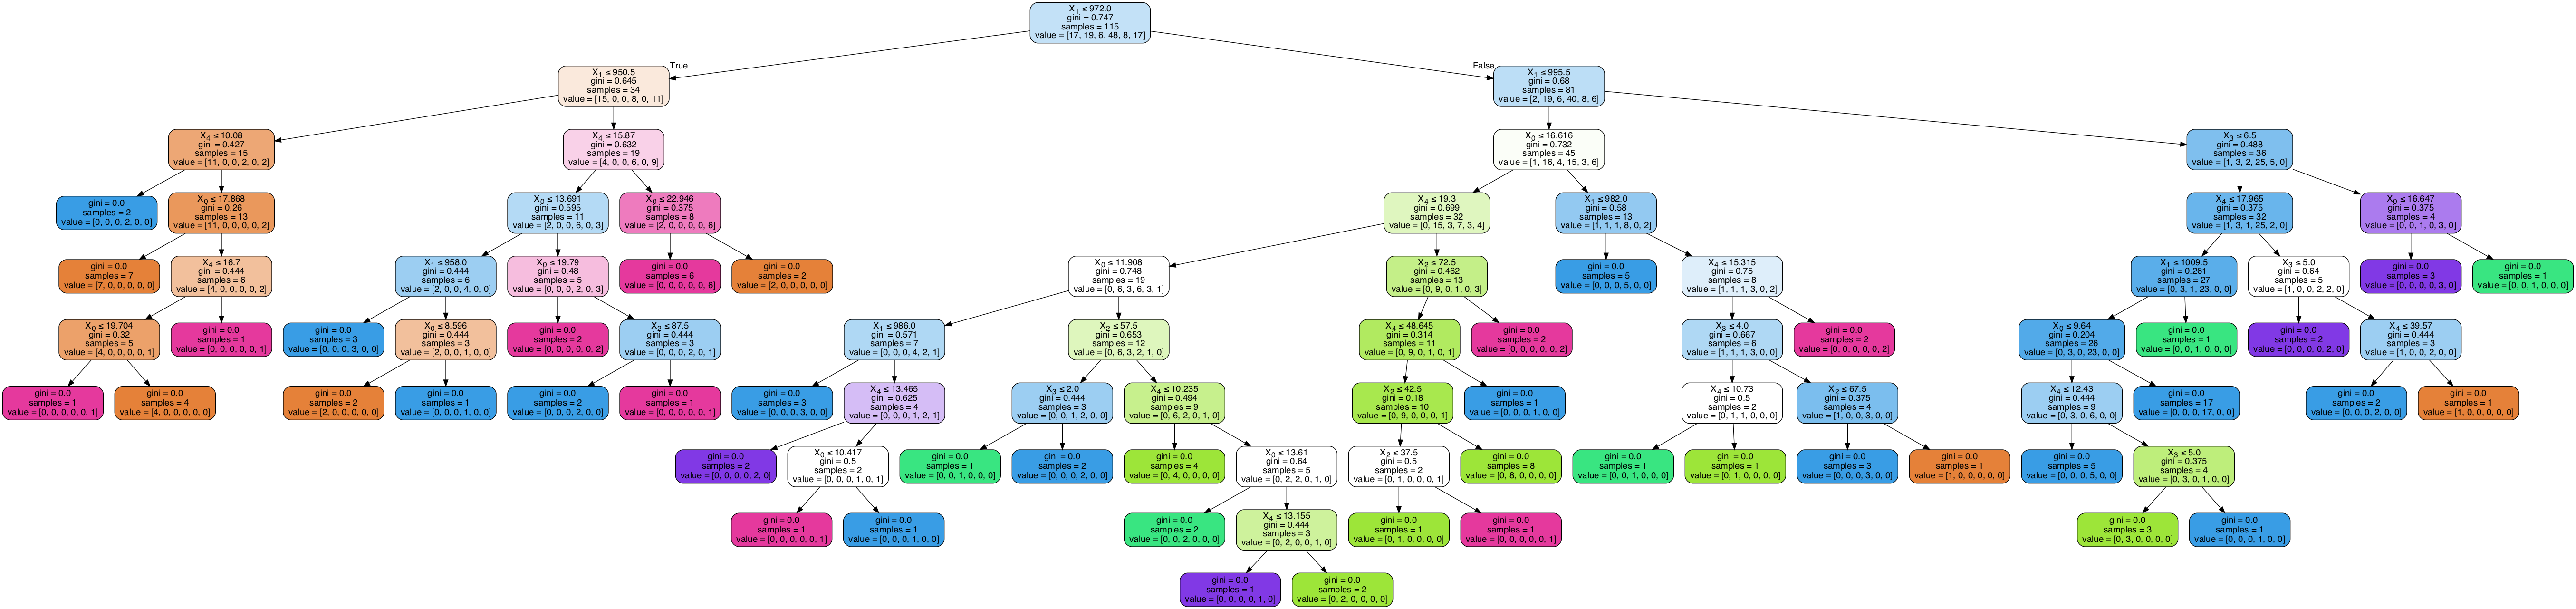
\includegraphics[width=\linewidth]{dtree.png}
  \caption{Decision Tree Visualization using Pydotplus package.}
  \label{fig:dtree}
\end{figure*}

\subsection{UNDERSTANDING DECISION TREE MODEL}
We used Decision Trees (DTs) as our optimal  predictive model as they are a non-parametric supervised learning method used for classification. Decision trees learn from data to approximate a sine curve with a set of if-then-else decision rules. The deeper the tree, the more complex the decision rules and the fitter the model gets. For  our model our optimal parameters for Decision tree was maximum\_depth = 10.

On plotting the decision tree as shown in Figure \ref{fig:dtree} We understand on how our model was able to classify values for storm events to be catastrophic or minimal.

The ‘value’ row in each node tells us how many of the observations that were sorted into that node fall into each of our 5 categories. We can see that our feature X4, which is the moon-phase, was able to completely distinguish one storm event type of catastrophic from the rest.

The biggest drawback to decision trees is that the split it makes at each node gets optimized for the data -set it is fit to. This splitting process will rarely generalize well to other data. However, in future work we can generate huge numbers of these decision trees, tuned in slightly different ways, and combine their predictions to create some of our best models for predicting storm damages today.

\section{CONCLUSION}	The initial goal of our study was to create a new scale and algorithm that could effectively predict the impact of a tropical weather system making landfall in the continental United States. We were able to show improvement over the Saffir-Simpson scale but were unable to reach our intended goal of at least 75\% accuracy. Further analysis will focus on tweaking some of the data parameters and finding ways to make the input data more comprehensive.


\section{References}
[1]B. Anderson, “Hurricaneexposuredata.” https://github.com/geanders/hurricaneexposure

[2]D. Gershgorn, “Artificial intelligence is great at predicting the size of hurricanes, but humans still need to figure out their impact,” Quartz. [Online]. Available: https://qz.com/1072215/artificial-intelligence-is-great-at-predicting-the-size-of-hurricanes-but-humans-still-need-to-figure-out-their-impact/. [Accessed: 28-Feb-2019].

[3]S. Giffard-Roisin, M. Yang, G. Charpiat, B. Kégl, and C. Monteleoni, “Fused Deep Learning for Hurricane Track Forecast from Reanalysis Data,” in Climate Informatics Workshop Proceedings 2018, Boulder, United States, 2018.

[4]T. Loridan, R. P. Crompton, and E. Dubossarsky, “A Machine Learning Approach to Modeling Tropical Cyclone Wind Field Uncertainty,” Mon. Wea. Rev., vol. 145, no. 8, pp. 3203–3221, May 2017.

[5]A. Sujithkumar, A. W. King, M. Kovilakam, and D. Graves, “Predicting the trajectories and intensities of hurricanes by applying machine learning techniques,” AGU Fall Meeting Abstracts, vol. 31, Dec. 2017.

[6]“Predicting Hurricane Damage with Machine Learning,” Datanami, 22-May-2017. [Online]. Available: https://www.datanami.com/2017/05/22/predicting-hurricane-damage-machine-learning/. [Accessed: 28-Feb-2019].

[7]“Detecting Storm Intensity from Satellite Imagery Using Machine Learning,” GIS Lounge, 11-Sep-2018. [Online]. Available: https://www.gislounge.com/detecting-storm-intensity-satellite-imagery-using-machine-learning/. [Accessed: 28-Feb-2019].

[8]“Consumer Price Index,” US Bureau of Labor Statistics.

[9]“Current Hurricane Data Sets.” [Online]. Available: http://www.aoml.noaa.gov/hrd/data\_sub/hurr.html. [Accessed: 28-Feb-2019].

[10]“GOES-East - Latest Full Disk Images - NOAA / NESDIS / STAR.” [Online]. Available: https://www.star.nesdis.noaa.gov/GOES/fulldisk.php?sat=G16. [Accessed: 28-Feb-2019].

[11]D. Roth. “Hurricane Point Rainfall Maxima.” https://www.wpc.ncep.noaa.gov/tropical/rain/tcmaxima.html

[12]“Methodology,” Deep Learning-based Hurricane Intensity Estimator. [Online]. Available: www.domain.org. [Accessed: 28-Feb-2019].

[13]“Past Atlantic Storm Tracks - Data.gov.” [Online]. Available: https://catalog.data.gov/dataset/past-atlantic-storm-tracks#topic=disasters-legacy\_navigation. [Accessed: 28-Feb-2019].

[14]“Storm Surge | U.S. Climate Resilience Toolkit.” [Online]. Available: https://toolkit.climate.gov/topics/coastal/storm-surge. [Accessed: 28-Feb-2019].


\end{document}
